\documentclass[11pt]{article}
% Shared preamble for the notes in this repository. pdfLaTeX, TeX Live 2024 or later.
\usepackage[a4paper,margin=2.6cm]{geometry}
\usepackage[T1]{fontenc}
\usepackage{lmodern}
\usepackage{microtype}
\usepackage{amsmath,amssymb,amsthm}
\usepackage{graphicx}
\usepackage{booktabs}
\usepackage{enumitem}
\usepackage[dvipsnames]{xcolor}
\usepackage[hidelinks]{hyperref}
\hypersetup{colorlinks=true,linkcolor=MidnightBlue,citecolor=MidnightBlue,urlcolor=MidnightBlue}
\graphicspath{{../../figures/}}
\setlist{itemsep=2pt,topsep=4pt}

\newtheorem{theorem}{Theorem}
\newtheorem{proposition}[theorem]{Proposition}
\newtheorem{corollary}[theorem]{Corollary}
\newtheorem{conjecture}[theorem]{Conjecture}
\theoremstyle{definition}
\newtheorem{definition}[theorem]{Definition}
% Reusable derivations, numbered note.k; each note sets \notenumber. Indexed in DERIVATIONS.md.
\newcommand{\notenumber}{0}
\newtheorem{derivation}{Derivation}
\renewcommand{\thederivation}{\notenumber.\arabic{derivation}}
\newtheorem{question}{Question}
\theoremstyle{remark}
\newtheorem{remark}[theorem]{Remark}

\newcommand{\Z}{\mathbb{Z}}
\newcommand{\Q}{\mathbb{Q}}
\newcommand{\R}{\mathbb{R}}
\newcommand{\C}{\mathbb{C}}
\newcommand{\HH}{\mathbb{H}}
\newcommand{\SL}{\mathrm{SL}}
\newcommand{\Gal}{\mathrm{Gal}}
\newcommand{\Hom}{\mathrm{Hom}}
\newcommand{\repo}{\href{https://github.com/rmorleysmith/l-functions-and-physics}{\texttt{l-functions-and-physics}}}
\newcommand{\formal}{\href{https://github.com/rmorleysmith/morley-smith-formal}{\texttt{morley-smith-formal}}}
\newcommand{\script}[1]{\href{https://github.com/rmorleysmith/l-functions-and-physics/blob/main/scripts/#1}{\texttt{scripts/#1}}}
% A path inside the Lean repository; it may break after a slash.
\newcommand{\leanpath}[1]{\nolinkurl{#1}}

% Grades used in every status table.
\newcommand{\gradeLean}{\textsc{lean}}      % proved in Lean 4 with Mathlib
\newcommand{\gradeClassical}{\textsc{classical}}  % a published theorem, cited
\newcommand{\gradeComputed}{\textsc{computed}}    % checked numerically by a script in this repository
\newcommand{\gradeConvention}{\textsc{convention}}  % a choice of units or names
\newcommand{\gradeOpen}{\textsc{open}}      % a question, conjecture or working hypothesis
% The legend printed under every status table.
\newcommand{\gradelegend}{\par\nopagebreak\smallskip\noindent\begin{minipage}{\textwidth}\small
\gradeLean: proved in Lean 4 with Mathlib.
\gradeClassical: a published theorem.
\gradeComputed: checked numerically by a script in the repository \repo.
\gradeConvention: a choice of units or names.
\gradeOpen: a question, conjecture or working hypothesis.
\end{minipage}\par\medskip}
% A plain-language physical reading, placed after each derivation.
\newcommand{\physical}{\paragraph{In physical terms.}}

\renewcommand{\notenumber}{13}

\title{Speed, spread and swirl:\\ motion on a lattice}
\author{Richard Morley-Smith}
\date{Note 13 \quad November 2026}

\begin{document}
\maketitle

\begin{abstract}
\noindent
We study three kinds of motion with objects from the earlier notes.
In special relativity in $2+1$ dimensions, the space of shapes of based lattices is the space of four-velocities, and the functional $S$ of note~12 is twice the relativistic kinetic energy of a body of mass $m$, in units of its rest energy $mc^2$.
The square lattice frame, moved by integral Lorentz transformations, reaches exactly the kinetic energies $\tfrac12 n\,mc^2$ for which $n$ and $n+4$ are both sums of two squares; this is proved in Lean.
On the axis of $\left(\begin{smallmatrix}2&1\\1&1\end{smallmatrix}\right)$, $n$ successive boosts have speed $\sqrt5F_{4n}/L_{4n}$, and Einstein's rule for adding velocities follows from the addition formulas of the Fibonacci and Lucas numbers.
For Burgers' equation of viscous flow, started by a lattice of point explosions, the Hopf--Cole substitution writes the velocity as $-2\nu\nabla\log\Theta$, with $\Theta$ the heat kernel of the torus, a theta function of the lattice: the fluid first fills the Voronoi cells of the lattice with Hubble flows, and at late times decays like its slowest tone.
For the Euler and Navier--Stokes equations in a periodic box, the flows built on one circle $|k|^2 = N$ in the plane form a space of dimension $r_2(N)$, and the Beltrami flows of one handedness built on one sphere $|k|^2 = N$ in space a space of dimension $r_3(N)$; for squarefree $N\not\equiv7\pmod8$ this is $(24/\pi)\sqrt N\,L(1,\chi_D)$, and it is zero exactly for $N = 4^a(8b+7)$.
Every computation is checked by a script.
\end{abstract}

\noindent
Throughout, $r_d(n)$ is the number of representations of $n$ as a sum of $d$ squares of integers, $\varphi = \tfrac12(1+\sqrt5)$, and for squarefree $N$, $D$ is the discriminant of $\Q(\sqrt{-N})$ and $\chi_D$ its quadratic character.
In the derivations speeds are in units of the speed of light; in the physical readings the speed of light is written $c$.

\section{Speed}

A positive definite symmetric matrix $A = \left(\begin{smallmatrix}\alpha&\beta\\\beta&\kappa\end{smallmatrix}\right)$ of determinant one is the point
\[
  (t,X,Y) = \bigl(\tfrac12(\alpha+\kappa),\ \tfrac12(\alpha-\kappa),\ \beta\bigr),\qquad t^2-X^2-Y^2 = \alpha\kappa-\beta^2 = 1,
\]
of the upper sheet of the unit hyperboloid of $2+1$ Minkowski space: the four-velocity of a body moving with velocity $(X/t,Y/t)$ relative to the frame of the identity matrix.
The normalised Gram matrix $M(z)$ of the based lattice $\Z+\Z z$ (note~12) is such a matrix, so the shape $z$ of a based lattice gives a four-velocity, and we call its rest frame the frame of $z$.
This is the picture of note~08, with the spatial axes exchanged: the upper half-plane is the space of velocities, and rapidity is hyperbolic distance \cite{RhodesSemon}.
A matrix $g = \left(\begin{smallmatrix}a&b\\c&d\end{smallmatrix}\right)\in\SL(2,\Z)$ acts by $A\mapsto gAg^{\mathsf T}$, a Lorentz transformation that preserves the integral matrices (an integral Lorentz transformation, note~08; $g$ and $-g$ act alike), and $gM(z)g^{\mathsf T} = M(gz)$.

\begin{derivation}[kinetic energy]\label{d:energy}
For two such matrices $A$, $B$, the Lorentz factor of one body seen from the other is
\[
  \gamma_{AB} = \tfrac12\,\mathrm{tr}\bigl(AB^{-1}\bigr) = \cosh\delta,
\]
where $\delta$ is the hyperbolic distance between the shapes, and the functional of note~12 is
\[
  \boxed{\;S(A,B) = \mathrm{tr}\bigl(AB^{-1}\bigr)-2-\log\det\bigl(AB^{-1}\bigr) = 2(\gamma_{AB}-1)\;}
\]
For speeds $v\ll1$, $S = v^2+\tfrac34v^4+O(v^6)$.
\end{derivation}

\noindent
Indeed $B^{-1} = \left(\begin{smallmatrix}\kappa'&-\beta'\\-\beta'&\alpha'\end{smallmatrix}\right)$, so $\mathrm{tr}(AB^{-1}) = \alpha\kappa'+\alpha'\kappa-2\beta\beta' = 2(tt'-XX'-YY')$, twice the Minkowski product of the two four-velocities, which is $\cosh\delta$ (Derivation~12.1); and $\det(AB^{-1}) = 1$.

\physical
A body of mass $m$ moving with Lorentz factor $\gamma$ has kinetic energy $(\gamma-1)mc^2$ \cite{Rindler}.
So $\tfrac12S\,mc^2$ is the kinetic energy of a body of mass $m$ at rest in the frame of one shape, measured in the frame of the other; for slow bodies it is $\tfrac12mv^2$ to leading order.
The square and hexagonal frames move relative to each other at $c/2$ (note~08): $\gamma = 2/\sqrt3$, and $S = 2(2/\sqrt3-1) = 0.309$ is the value found in note~12.

\begin{derivation}[the energies of the square frame]\label{d:square}
For $g = \left(\begin{smallmatrix}a&b\\c&d\end{smallmatrix}\right)\in\SL(2,\Z)$,
\[
  S\bigl(M(i),M(gi)\bigr) = (a-d)^2+(b+c)^2,\qquad S+4 = (a+d)^2+(b-c)^2 .
\]
The values taken are exactly the $n\ge0$ for which $n$ and $n+4$ are both sums of two squares: $0, 1, 4, 5, 9, 13, 16, 25, 32, 36, 37, 41,\dots$
The number of matrices $g$ with $S = n$ is $r_2(n)\,r_2(n+4)$ for $n\equiv0\pmod 4$ and half of it for odd $n$.
\end{derivation}

\noindent
Proof.
Since $M(i) = I$ and $M(gi) = gg^{\mathsf T}$, $\mathrm{tr}(M(i)M(gi)^{-1}) = \mathrm{tr}\,gg^{\mathsf T} = a^2+b^2+c^2+d^2$, and the two displayed identities follow from $ad-bc = 1$; so every value has the stated property.
Conversely, let $n = p^2+q^2$ and $n+4 = r^2+s^2$ with $r\equiv p$ and $s\equiv q\pmod 2$; then $a = \tfrac12(r+p)$, $d = \tfrac12(r-p)$, $b = \tfrac12(q+s)$, $c = \tfrac12(q-s)$ are integers with $ad-bc = \tfrac14(r^2+s^2-p^2-q^2) = 1$.
The parities can always be matched, because $n\equiv0$ or $1\pmod4$ whenever $n$ and $n+4$ are both sums of two squares: a number $\equiv3\pmod4$ is not a sum of two squares, and for $n = 2m$ with $m$ odd, $n$ and $n+4$ are sums of two squares only if $m$ and $m+2$ are, and one of these is $\equiv3\pmod4$.
If $n\equiv0\pmod4$, all of $p,q,r,s$ are even; if $n\equiv1\pmod4$, exactly one of $p,q$ and exactly one of $r,s$ is odd, and exchanging $r$ and $s$ if necessary matches them.
The map $g\mapsto(a-d,\,b+c,\,a+d,\,b-c)$ is a bijection from the $g$ with $S = n$ onto the quadruples with $p^2+q^2 = n$, $r^2+s^2 = n+4$, $p\equiv r$ and $q\equiv s\pmod 2$.
For odd $n$, half of the representations of $n$ have $p$ odd and half of those of $n+4$ have $r$ odd, so half of the pairs qualify.
The identities and the description of the values are proved in Lean in \formal{} (\leanpath{MorleySmithFormal/SquareFrameEnergies}).

\physical
Moving the square frame by integral Lorentz transformations, one reaches only the kinetic energies $\tfrac12 n\,mc^2$ with $n$ and $n+4$ sums of two squares: the two-squares condition applied twice (Figure~\ref{fig:speed}).
The four matrices $\pm I$, $\pm\left(\begin{smallmatrix}0&-1\\1&0\end{smallmatrix}\right)$, the rotations of the square lattice, fix it ($n = 0$); the nearest moving frames have $n = 1$ and speed $(\sqrt5/3)\,c$; the energies $n = 2, 3, 6, 7, 8, 10,\dots$ never occur.
The number of matrices reaching the energy $\tfrac12n\,mc^2$ is $r_2(n)\,r_2(n+4)$, halved for odd $n$, and $r_2(n)$ is the $n$-th coefficient of $4\zeta(s)L(s,\chi_{-4})$ (note~02).
The number of matrices with $S\le X$ grows like $6X$, the hyperbolic lattice-point problem at $z = i$ \cite{Iwaniec}; the script finds $5.9994\,X$ at $X = 2\cdot10^5$.

\begin{figure}[ht]
  \centering
  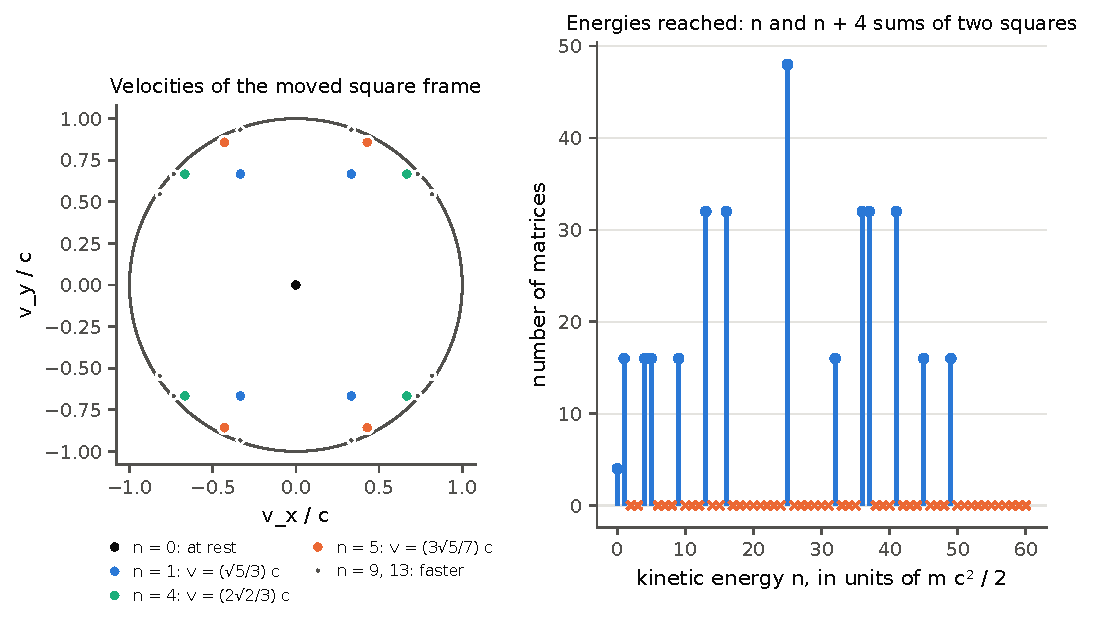
\includegraphics[width=0.96\textwidth]{motion-velocities}
  \caption{Left: the velocities of the square frame after the integral Lorentz transformations with $n\le13$; each point is reached by four matrices. Right: the number of matrices reaching each kinetic energy $\tfrac12n\,mc^2$, with the energies that never occur marked.}
  \label{fig:speed}
\end{figure}

\begin{derivation}[golden boosts]\label{d:golden}
The matrix $g = \left(\begin{smallmatrix}2&1\\1&1\end{smallmatrix}\right)$ has eigenvalues $\varphi^{\pm2}$, and its axis is the semicircle with endpoints $\tfrac12(1\pm\sqrt5)$, which passes through $i$.
On its axis, $g$ moves every frame with Lorentz factor $\tfrac72$, speed $3\sqrt5/7$ and rapidity
\[
  \eta = 4\log\varphi = 2\sqrt5\,L(1,\chi_5),
\]
and its $n$-th power with Lorentz factor $\tfrac12L_{4n}$ and speed $v_n = \sqrt5\,F_{4n}/L_{4n}$, where $F$ and $L$ are the Fibonacci and Lucas numbers.
Einstein's rule for adding collinear velocities, $v_{m+n} = (v_m+v_n)/(1+v_mv_n)$, follows for these speeds by dividing the addition formulas
\[
  2F_{a+b} = F_aL_b+F_bL_a,\qquad 2L_{a+b} = L_aL_b+5F_aF_b,
\]
with $a = 4m$ and $b = 4n$.
Every hyperbolic element of $\SL(2,\Z)$ gives every frame a Lorentz factor of at least $\tfrac72$.
\end{derivation}

\noindent
The rapidity on the axis is $\eta = 2\log\varphi^2$, so $v_n = \tanh n\eta = (\varphi^{4n}-\varphi^{-4n})/(\varphi^{4n}+\varphi^{-4n})$, which is $\sqrt5F_{4n}/L_{4n}$ by Binet's formulas \cite{Vajda}.
The value $L(1,\chi_5) = (2/\sqrt5)\log\varphi$ is Dirichlet's class number formula for $\Q(\sqrt5)$, with class number one and fundamental unit $\varphi$ \cite{Davenport}.
The last statement is $S\ge5$ for hyperbolic elements, Derivation~12.2, proved in Lean in \formal{} (\leanpath{MorleySmithFormal/LatticeMetricDivergence}).

\physical
No integral boost is slow: a hyperbolic integral Lorentz transformation takes every frame to one receding from it at a speed of at least $3\sqrt5/7\,c = 0.958\,c$, and the golden boost, like every element of trace $\pm3$, does so exactly on its axis.
The rapidity of that slowest boost is the length of the shortest closed geodesic of the modular surface (note~05), and it equals $2\sqrt5\,L(1,\chi_5)$.
Two golden boosts give $21\sqrt5/47\,c = 0.99909\,c$.
The parabolic elements are null rotations, and they move frames arbitrarily slowly: $\left(\begin{smallmatrix}1&1\\0&1\end{smallmatrix}\right)$ moves $z = x+iy$ with $S = 1/y^2$, which tends to $0$ as $y\to\infty$ (note~12).

\section{Spread}

\begin{derivation}[heat on a lattice]\label{d:heat}
For a lattice $\Lambda\subset\R^d$ of covolume $V$ with dual lattice $\Lambda^*$, the solution of $\partial_t\Theta = \nu\Delta\Theta$ with initial value a unit point mass at every lattice point, $\Theta(\cdot,0) = \sum_{n\in\Lambda}\delta_n$, is
\[
  \Theta(x,t) = \sum_{n\in\Lambda}\frac{e^{-|x-n|^2/4\nu t}}{(4\pi\nu t)^{d/2}} = \frac1V\sum_{k\in\Lambda^*}e^{-4\pi^2\nu t|k|^2}\,e^{2\pi i\langle k,x\rangle}.
\]
\end{derivation}

\noindent
The two sums are equal by Poisson summation (note~07); the first converges rapidly at short times and the second at long times.

\physical
At short times the heat is the sum of the spreading images of the point masses; at long times it is the sum of the tones (Laplace eigenmodes) of the torus $\R^d/\Lambda$, each decaying at the rate $4\pi^2\nu|k|^2$.
For $\Lambda = \Z^3$ the tone $|k|^2 = N$ has multiplicity $r_3(N)$, and there is no tone at the empty shells of note~11.

\begin{derivation}[a lattice of explosions]\label{d:burgers}
Burgers' equation for a velocity field $u = \nabla\psi$,
\[
  \partial_tu+(u\cdot\nabla)u = \nu\Delta u,
\]
is turned into the heat equation by the substitution $u = -2\nu\nabla\log\Theta$ of Hopf and Cole \cite{Hopf, Cole}.
With $\Theta$ as in Derivation~\ref{d:heat},
\[
  \boxed{\;u(x,t) = \frac{x-\langle n\rangle}{t},\qquad \langle n\rangle = \frac{\sum_{n\in\Lambda}n\,e^{-|x-n|^2/4\nu t}}{\sum_{n\in\Lambda}e^{-|x-n|^2/4\nu t}}\;}
\]
As $\nu t\to0$, $\langle n\rangle$ tends to the lattice point nearest to $x$, away from the walls of the Voronoi cells of $\Lambda$; at late times $u$ decays like $e^{-4\pi^2\nu|k|^2t}$, with $k$ a shortest nonzero vector of $\Lambda^*$.
\end{derivation}

\physical
The equation appears in Bateman's work on fluid motion \cite{Bateman}; Burgers studied it as a model of turbulence \cite{Burgers}.
Here every lattice point explodes at $t = 0$.
At first each Voronoi cell (in crystallography, the Wigner--Seitz cell) holds its own Hubble flow $u = r/t$, centred on its own point, and the flows meet at thin viscous shocks on the cell walls: squares for the square lattice and hexagons for the hexagonal one (Figure~\ref{fig:burgers}); in space, cubes for $\Z^3$, rhombic dodecahedra for the face-centred cubic lattice and truncated octahedra for the body-centred one \cite{ConwaySloane}.
At late times the faster tones have died out and the flow decays like its slowest tone.
In the limit $\nu\to0$ and with a random initial velocity potential in place of the lattice, the same equation is the adhesion model of the large-scale structure of the Universe, in which matter collects on the walls, edges and vertices of a tessellation of space \cite{GSS}.

\begin{figure}[ht]
  \centering
  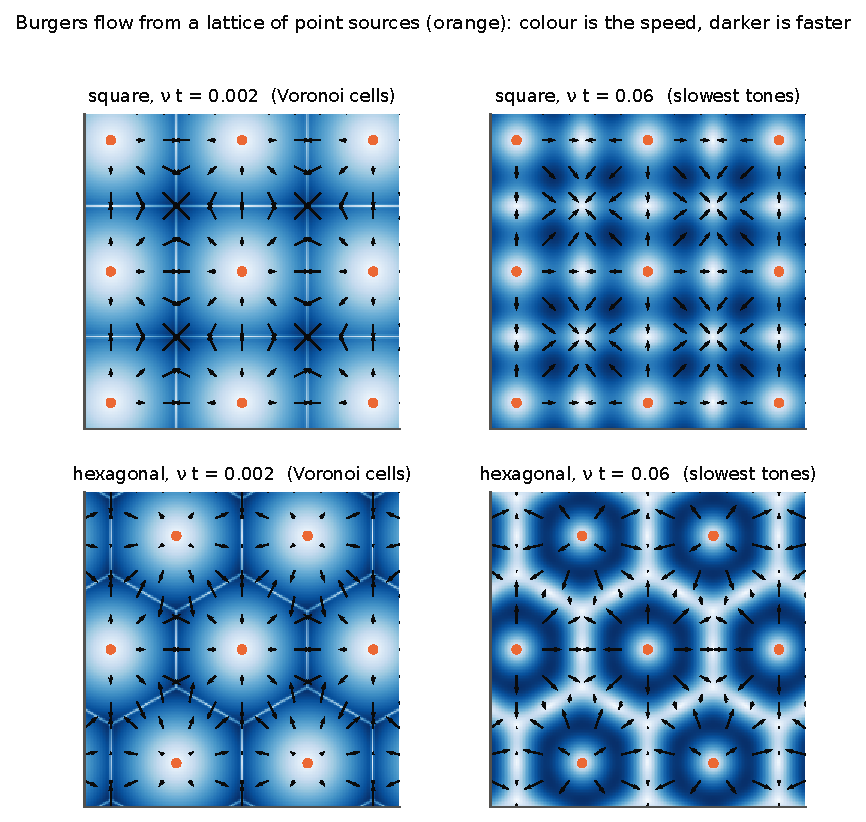
\includegraphics[width=0.74\textwidth]{motion-burgers}
  \caption{Burgers flow from a lattice of point explosions (orange); the pattern depends only on $\nu t$. Left: at $\nu t = 0.002$ the flow fills the Voronoi cells, with shocks on their walls. Right: at $\nu t = 0.06$ the slowest tones remain.}
  \label{fig:burgers}
\end{figure}

\section{Swirl}

\begin{derivation}[cellular flows in a periodic plane box]\label{d:cellular}
On $\R^2/\Z^2$ let $\psi = \sum_{|k|^2 = N}c_k\,e^{2\pi i\langle k,x\rangle}$ with $c_{-k} = \overline{c_k}$, and $u = (\partial_y\psi,-\partial_x\psi)$.
The vorticity is $\omega = -\Delta\psi = 4\pi^2N\psi$, so $u\cdot\nabla\omega = 0$: $u$ is a steady flow of the Euler equations, and since $\Delta u = -4\pi^2Nu$ it decays exactly as $e^{-4\pi^2\nu Nt}$ under the Navier--Stokes equations with viscosity $\nu$.
These flows form a real vector space of dimension
\[
  r_2(N) = 4\sum_{d\mid N}\chi_{-4}(d),
\]
which is zero exactly when a prime $\equiv3\pmod4$ divides $N$ to an odd power \cite{Grosswald}.
\end{derivation}

\noindent
These are the decaying vortex arrays of Taylor \cite{Taylor1923}; the case $N = 2$ contains the two-dimensional Taylor--Green vortex $\psi = \sin2\pi x\,\sin2\pi y$ \cite{TaylorGreen}.

\begin{derivation}[Beltrami flows in a periodic cubic box]\label{d:beltrami}
On $\R^3/\Z^3$ let $u = \sum_{|k|^2 = N}a_k\,e^{2\pi i\langle k,x\rangle}$ with $a_{-k} = \overline{a_k}$, each $a_k$ orthogonal to $k$ and of positive helicity, $i\,(k/|k|)\times a_k = a_k$.
Then $\nabla\times u = 2\pi\sqrt N\,u$: the velocity is parallel to the vorticity, a Beltrami field \cite{Beltrami}, and
\[
  (u\cdot\nabla)u = \nabla\tfrac12|u|^2-u\times(\nabla\times u) = \nabla\tfrac12|u|^2,
\]
so $u$ is a steady flow of the Euler equations with pressure $-\tfrac12|u|^2$, and since $\Delta u = -4\pi^2Nu$ it decays exactly as $e^{-4\pi^2\nu Nt}$ under the Navier--Stokes equations \cite{Trkal}.
These flows form a real vector space of dimension $r_3(N)$, the same for negative helicity; for squarefree $N\not\equiv7\pmod 8$
\[
  \boxed{\;r_3(N) = \frac{24}{\pi}\sqrt N\,L(1,\chi_D)\;}
\]
(note~11), and $r_3(N) = 0$ exactly for $N = 4^a(8b+7)$, by the theorem of Legendre and Gauss \cite{Grosswald}.
\end{derivation}

\noindent
The case $N = 1$ has $r_3(1) = 6$ real parameters: for each coordinate axis, one amplitude and one phase of a helical wave along that axis.
Translations shift the three phases independently, so this family consists of the ABC flows of Arnold and Childress and their translates \cite{Arnold, Childress}; their streamlines can be chaotic, as Hénon found numerically \cite{Henon} and Dombre et al.\ studied in detail \cite{Dombre}.

\physical
An ideal fluid in a periodic cubic box has, for each handedness, an $r_3(N)$-dimensional space of steady Beltrami flows built on the wavenumber $2\pi\sqrt N$.
Its dimension is the number of lattice points on the sphere of radius $\sqrt N$, the strength of the $N$-th echo of note~11 up to the factor $4\pi\sqrt N$; for squarefree $N\not\equiv7\pmod8$ it equals $(24/\pi)\sqrt N\,L(1,\chi_D)$.
At $N = 7, 15, 23, 28,\dots$ there is no such flow.
In the plane the count is $r_2(N)$, and there is none at $N = 3, 6, 7, 11, 12,\dots$ (Figure~\ref{fig:swirl}).
Under viscosity each of these flows decays exponentially without changing its shape.

\begin{figure}[ht]
  \centering
  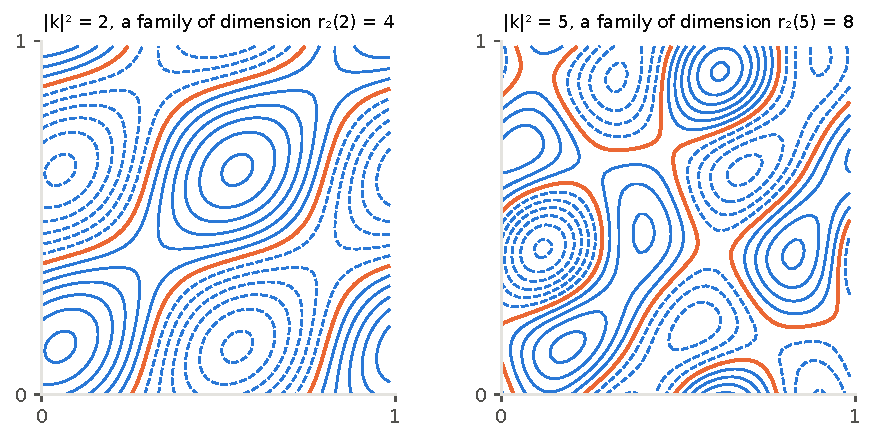
\includegraphics[width=0.8\textwidth]{motion-swirl}
  \caption{Streamlines of two exact cellular flows in a periodic plane box, with random coefficients on the circles $|k|^2 = 2$ and $|k|^2 = 5$. The zero streamline is orange.}
  \label{fig:swirl}
\end{figure}

\section*{Status of the statements}

\begin{center}
\small
\begin{tabular}{@{}p{0.66\textwidth}l@{}}
\toprule
Statement & Grade\\
\midrule
The hyperboloid model of velocity space (note~08) \cite{PenroseRindler, RhodesSemon}; kinetic energy $(\gamma-1)mc^2$ \cite{Rindler} & \gradeClassical, \gradePhysics\\
Derivation~\ref{d:energy}: $\gamma_{AB} = \tfrac12\mathrm{tr}(AB^{-1})$ and $S = 2(\gamma_{AB}-1)$ on lattice metrics (Derivation~12.1); 100 random pairs & \gradeLean, \gradeComputed\\
Derivation~\ref{d:square}: the identities and the values of $S$ (\leanpath{MorleySmithFormal/SquareFrameEnergies}); all $n\le60$ & \gradeLean, \gradeComputed\\
Derivation~\ref{d:square}: the count $r_2(n)r_2(n+4)$ (proved above; $n\le60$); growth $6X$ \cite{Iwaniec} & \gradeClassical, \gradeComputed\\
Derivation~\ref{d:golden}: speeds, rapidity and the Fibonacci--Lucas identities \cite{Vajda, Davenport}; $i$ and 20 points on the axis & \gradeClassical, \gradeComputed\\
Derivation~\ref{d:golden}: Lorentz factor at least $\tfrac72$ for hyperbolic elements (Derivation~12.2); equality on the axes of trace $\pm3$ & \gradeLean, \gradeComputed\\
Derivation~\ref{d:heat}: Poisson summation; checked on the circle and the hexagonal torus & \gradeClassical, \gradeComputed\\
Derivation~\ref{d:burgers}: the Hopf--Cole solution, the Voronoi limit and the slowest tone (square and hexagonal); the cells of the cubic lattices \cite{ConwaySloane} & \gradeClassical, \gradeComputed\\
Derivations~\ref{d:cellular} and~\ref{d:beltrami}: the Euler property, checked spectrally for $N = 1, 2, 5, 25, 65$ (plane) and $N = 1, 2, 3, 5, 6$ (space); the Navier--Stokes decay from $\Delta u = -4\pi^2Nu$ \cite{Taylor1923, Trkal} & \gradeClassical, \gradeComputed\\
The dimensions $r_2(N)$ and $r_3(N)$, their zero sets, and $r_3(N) = (24/\pi)\sqrt N\,L(1,\chi_D)$ (Jacobi, Legendre, Gauss, Dirichlet \cite{Grosswald, Davenport}); $N\le50$ & \gradeClassical, \gradeComputed\\
The adhesion model \cite{GSS}; chaotic ABC streamlines \cite{Henon, Dombre} & \gradePhysics, \gradeClassical\\
\bottomrule
\end{tabular}
\end{center}
\gradelegend

\begin{sloppypar}\noindent
All checks are in \script{motion\_and\_flow.py}.
\end{sloppypar}

\begin{thebibliography}{99}\small
\bibitem{Arnold} V.~I. Arnold, Sur la topologie des \'ecoulements stationnaires des fluides parfaits, \emph{C. R. Acad. Sci. Paris} 261 (1965), 17--20.
\bibitem{Bateman} H.~Bateman, Some recent researches on the motion of fluids, \emph{Monthly Weather Review} 43 (1915), 163--170.
\bibitem{Beltrami} E.~Beltrami, Considerazioni idrodinamiche, \emph{Il Nuovo Cimento} (3) 25 (1889), 212--222.
\bibitem{Burgers} J.~M. Burgers, A mathematical model illustrating the theory of turbulence, \emph{Adv. Appl. Mech.} 1 (1948), 171--199.
\bibitem{Childress} S.~Childress, New solutions of the kinematic dynamo problem, \emph{J. Math. Phys.} 11 (1970), 3063--3076.
\bibitem{Cole} J.~D. Cole, On a quasi-linear parabolic equation occurring in aerodynamics, \emph{Quart. Appl. Math.} 9 (1951), 225--236.
\bibitem{ConwaySloane} J.~H. Conway and N.~J.~A. Sloane, \emph{Sphere Packings, Lattices and Groups}, 3rd ed., Springer, 1999.
\bibitem{Davenport} H.~Davenport, \emph{Multiplicative Number Theory}, 3rd ed., revised by H.~L. Montgomery, Graduate Texts in Mathematics 74, Springer, 2000.
\bibitem{Dombre} T.~Dombre, U.~Frisch, J.~M. Greene, M.~H\'enon, A.~Mehr and A.~M. Soward, Chaotic streamlines in the ABC flows, \emph{J. Fluid Mech.} 167 (1986), 353--391.
\bibitem{Grosswald} E.~Grosswald, \emph{Representations of Integers as Sums of Squares}, Springer, 1985.
\bibitem{GSS} S.~N. Gurbatov, A.~I. Saichev and S.~F. Shandarin, The large-scale structure of the Universe in the frame of the model equation of non-linear diffusion, \emph{Mon. Not. R. Astron. Soc.} 236 (1989), 385--402.
\bibitem{Henon} M.~H\'enon, Sur la topologie des lignes de courant dans un cas particulier, \emph{C. R. Acad. Sci. Paris} 262 (1966), 312--314.
\bibitem{Hopf} E.~Hopf, The partial differential equation $u_t+uu_x = \mu u_{xx}$, \emph{Comm. Pure Appl. Math.} 3 (1950), 201--230.
\bibitem{Iwaniec} H.~Iwaniec, \emph{Spectral Methods of Automorphic Forms}, 2nd ed., American Mathematical Society, 2002.
\bibitem{PenroseRindler} R.~Penrose and W.~Rindler, \emph{Spinors and Space-Time}, vol.~1, Cambridge University Press, 1984.
\bibitem{RhodesSemon} J.~A. Rhodes and M.~D. Semon, Relativistic velocity space, Wigner rotation, and Thomas precession, \emph{Amer. J. Phys.} 72 (2004), 943--960.
\bibitem{Rindler} W.~Rindler, \emph{Relativity: Special, General, and Cosmological}, 2nd ed., Oxford University Press, 2006.
\bibitem{Taylor1923} G.~I. Taylor, On the decay of vortices in a viscous fluid, \emph{Phil. Mag.} (6) 46 (1923), 671--674.
\bibitem{TaylorGreen} G.~I. Taylor and A.~E. Green, Mechanism of the production of small eddies from large ones, \emph{Proc. R. Soc. Lond. A} 158 (1937), 499--521.
\bibitem{Trkal} V.~Trkal, A remark on the hydrodynamics of the viscous fluids, \emph{\v{C}asopis pro p\v{e}stov\'an\'i matematiky a fysiky} 48 (1919), 302--311 (in Czech); English translation: A note on the hydrodynamics of viscous fluids, \emph{Czech. J. Phys.} 44 (1994), 97--106.
\bibitem{Vajda} S.~Vajda, \emph{Fibonacci and Lucas Numbers, and the Golden Section}, Ellis Horwood, 1989.
\end{thebibliography}

\end{document}
